\begin{figure}[H]
\centering
\resizebox{\textwidth}{!}{%
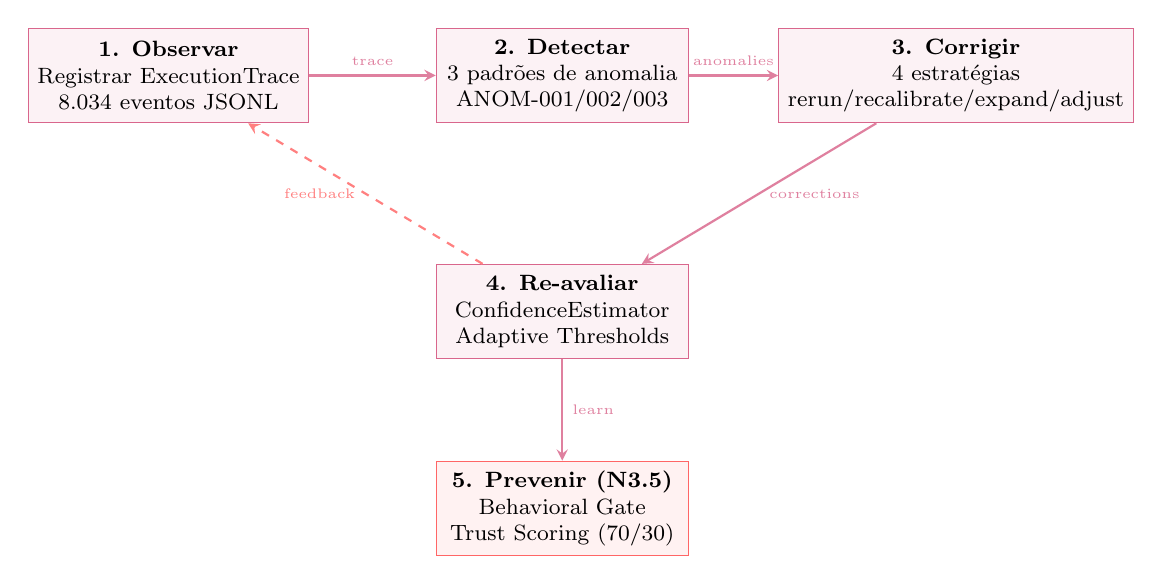
\begin{tikzpicture}[
    box/.style={rectangle, draw=purple!60, fill=purple!5, minimum width=3.2cm, minimum height=1.2cm, align=center, font=\footnotesize},
    arrow/.style={->, >=stealth, thick, purple!50},
    loop/.style={->, >=stealth, thick, red!50, dashed},
]
\node[box] (OBS) at (0,2) {\textbf{1. Observar}\\Registrar ExecutionTrace\\8.034 eventos JSONL};
\node[box] (DET) at (5,2) {\textbf{2. Detectar}\\3 padrões de anomalia\\ANOM-001/002/003};
\node[box] (COR) at (10,2) {\textbf{3. Corrigir}\\4 estratégias\\rerun/recalibrate/expand/adjust};
\node[box] (REAV) at (5,-1) {\textbf{4. Re-avaliar}\\ConfidenceEstimator\\Adaptive Thresholds};

\draw[arrow] (OBS) -- (DET) node[midway,above,font=\tiny] {trace};
\draw[arrow] (DET) -- (COR) node[midway,above,font=\tiny] {anomalies};
\draw[arrow] (COR) -- (REAV) node[midway,right,font=\tiny] {corrections};
\draw[loop] (REAV) -- (OBS) node[midway,left,font=\tiny] {feedback};

\node[box,draw=red!60,fill=red!5] (GATE) at (5,-3.5) {\textbf{5. Prevenir (N3.5)}\\Behavioral Gate\\Trust Scoring (70/30)};
\draw[arrow] (REAV) -- (GATE) node[midway,right,font=\tiny] {learn};
\end{tikzpicture}%
}
\caption{Ciclo Metacognitivo completo — Observar $\rightarrow$ Detectar $\rightarrow$ Corrigir $\rightarrow$ Re-avaliar $\rightarrow$ Prevenir. O feedback loop (seta tracejada) garante que cada correção seja re-avaliada. O Behavioral Gate (N3.5) fecha o ciclo aprendendo com os outcomes para prevenir ações de baixa confiança.}
\label{fig:metacognicao}
\end{figure}
